\documentclass[10pt]{article}
\usepackage[margin=1in]{geometry}
\usepackage{times}
\usepackage[T1]{fontenc}
\usepackage{amsmath,amssymb,amsthm}
\usepackage{booktabs}
\usepackage{graphicx}
\usepackage{microtype}
\usepackage[numbers,sort&compress]{natbib}
\usepackage{xcolor}
\usepackage[colorlinks=true,linkcolor=blue!50!black,citecolor=blue!50!black,urlcolor=blue!50!black]{hyperref}
\usepackage[capitalise,noabbrev]{cleveref}

\newtheorem{proposition}{Proposition}
\newcommand{\sps}{\textsc{sps}}
\newcommand{\shat}{\hat{s}}

\title{Sim2Real Without the Sim: Lessons from a Top-10 Entry\\in the NeurIPS 2026 RealPDE Challenge}
\author{Junlong Shen\\University of Alberta, Edmonton, Canada\\\texttt{junlong6@ualberta.ca}}
\date{}

\begin{document}
\maketitle

\begin{abstract}
We describe our entry to Track~1 (Sim2Real) of the NeurIPS 2026 RealPDE Challenge, which asks for 20-frame forecasts of real particle-image-velocimetry (PIV) measurements of flow past a foil, with per-element uncertainty intervals, scored on accuracy, turbulence statistics, interval quality and latency. The entry placed 9th of the finalists after the organizers retrained every finalist's code on a private set of unseen flow conditions (final score $82.31\pm0.006$). It uses no simulation data: four 1.2M-parameter 2-D convolutional operators trained on 81 real trajectories, physically exact Reynolds-similarity augmentation, and a post-hoc width table fitted to maximise the challenge's interval reward. The paper's main content is what 440 logged experiments and 22 hidden-test submissions say about this regime. (i) The interval score has a closed-form per-element optimum whose coverage depends on the residual scale, so it rewards abandoning hard elements. Getting this calibration right separated the top of the field from the median more than forecast accuracy did. A single width-table refit, with predictions bit-identical, was worth $+0.78$ on the hidden test, more than any modelling change after the first week. (ii) Simulation data did not help: pretrain-then-finetune was neutral, and joint training lost monotonically with the simulation fraction, even after simulating the PIV measurement process. (iii) The model is limited by independent real trajectories and by phase error, not by capacity or fluctuation amplitude. We release the code and the negative results, each with its oracle bound or dose-response.
\end{abstract}

\section{Introduction}

Scientific machine learning for partial differential equations is usually trained and evaluated on simulations. RealPDEBench~\citep{hu2026realpdebench} pairs real measurements with matched simulations and reports that pretraining on simulated data improves accuracy and convergence on the real data. The NeurIPS 2026 RealPDE Challenge~\citep{realpde2026competition} builds on it. Its Track~1, \emph{Sim2Real}, releases real PIV recordings of flow past a foil together with a larger simulated corpus and scores 20-frame forecasts on a hidden real test set. The final ranking was decided by the organizers retraining each finalist's submitted code on a private set of unseen (angle of attack, Reynolds number) conditions.

Our entry ranked 9th of the ten finalists (\cref{tab:final}), without any cash prize or co-authorship of the organizers' summary paper. We write this report for two reasons. First, the entry uses no simulation data at all, and we have controlled evidence that simulation data did not help, which bears directly on the track's premise. Second, the competition record is unusually complete: 440 logged experiments, each with a stated falsifier, controls and noise floor; 160 named \emph{levers} (candidate improvements), 101 of them ruled out with evidence; and 22 hidden-test submissions, several of which change exactly one thing. Negative results with oracle bounds are rarely published, and they are what a later team needs most.

\paragraph{Contributions.}
\begin{itemize}
\item An analysis of the challenge's interval score (\sps{}) showing that its optimum is a per-element closed form whose coverage falls with the residual scale (\cref{sec:sps}), and a non-parametric width table that attains it to within $0.0007$ of the reward of its own class oracle (\cref{sec:width}).
\item Evidence from the leaderboard that interval calibration, not forecast accuracy, separated the top of the field from the median (\cref{sec:where}), and a hidden-test measurement in which a width-table refit alone, with identical predictions, gained $+0.78$ final score.
\item Controlled negative results on simulation data: pretraining, joint training and measurement-process degradation (\cref{sec:sim}).
\item A characterisation of the real-data regime: data-limited in independent trajectories, insensitive to capacity over a $12\times$ range, improved by physically exact Reynolds-similarity augmentation, and limited by phase rather than amplitude error (\cref{sec:regime,sec:phase}).
\item The released training and inference code, which reproduces the submitted entry from the public data alone.
\end{itemize}

\section{Task, data and metric}
\label{sec:task}

\paragraph{Data.} The real training set holds 81 PIV trajectories of the two in-plane velocity components $(u,v)$ behind a foil, at five angles of attack and Reynolds numbers spanning a factor of $9.4$. One further released file duplicates another and is excluded. Following the organizers' loader we subsample the $64\times128$ grid to $32\times64$, which gives 69,085 frames. About 10\% of every frame is zero where the laser sheet is obstructed; the scorer excludes target zeros from the interval score. The simulated set holds 100 trajectories (100,000 frames) with pressure, including two Reynolds numbers absent from the real set. The simulated $u$ and $v$ have $3.9\times$ and $15\times$ the standard deviation of the real ones.

\paragraph{Task.} Given 20 input frames, predict the next 20 frames of $(u,v)$ together with a lower and upper bound per element. Predictions are made per window; pooling statistics across the windows of one call is forbidden.

\paragraph{Scores.} Five sub-scores are computed on the hidden set. With $e$ a per-window relative error, accuracy scores map $e\mapsto 100/(1+e/2)$: \emph{rel\_l2} is the relative $L_2$ error of the field; \emph{tke} is the relative error of the per-pixel temporal variance (turbulent kinetic energy) map; \emph{mvpe} is the relative error of the time-mean velocity at 36 wake probes. \emph{time} is $100/(1+\sqrt{t/0.729})$ for $t$ the charged milliseconds per sample on a shared evaluation host. The interval score is
\begin{equation}
\sps = 100\sum_{b} w_b\,\frac{1}{|\mathcal{S}|}\sum_{i\in\mathcal{S}} (1-p_{b,n(i)})\, e^{-(U_i-L_i)/\sigma}\,\mathbf{1}\{L_i\le y_i\le U_i\},
\label{eq:sps}
\end{equation}
where $\mathcal{S}$ is the set of non-zero target elements, $\sigma=0.0564$, and the three branches $b$ (weights $0.5,0.3,0.2$) use a per-window penalty $p=e/(0.5+e)$ from the rel\_l2, tke and mvpe errors of window $n(i)$. The organizers did not publish the aggregation into the final score. A linear fit to 22 of our own scored rows gives weights rel\_l2 $0.466$, \sps{} $0.246$, mvpe $0.105$, tke $0.102$, time $0.096$, with leave-one-out error $0.008$; it reproduces the top-10 board to $0.002$. We use these weights only to attribute differences.

\subsection{The interval score has a closed-form, non-quantile optimum}
\label{sec:sps}

The factor $(1-p)$ in \cref{eq:sps} depends only on the point prediction, and every element enters independently. The choice of interval therefore decouples per element.

\begin{proposition}
Fix the point prediction $\mu_i$. For a symmetric interval $[\mu_i-h,\mu_i+h]$ and residual $r_i=y_i-\mu_i$ with conditional law $P_i$, the expected contribution of element $i$ is proportional to $F_i(h)=e^{-2h/\sigma}\,P_i(|r_i|\le h)$, so the optimal interval is $h_i^\star=\arg\max_h F_i(h)$, independently of every other element. If $r_i\sim\mathcal{N}(0,s_i^2)$, then $h_i^\star=k^\star(s_i/\sigma)\,s_i$, where $k^\star$ solves $(\sigma/s_i)\,\varphi(k)=\operatorname{erf}(k/\sqrt2)$, and the optimal coverage $\operatorname{erf}(k^\star/\sqrt2)$ decreases from $1$ to $0$ as $s_i/\sigma$ grows.
\end{proposition}
\begin{proof}
Differentiate $\log F_i$: $-2/\sigma+2\varphi(h/s_i)/(s_i\operatorname{erf}(h/(s_i\sqrt2)))=0$. The left side of the stated equation is decreasing in $k$ and the right side increasing, so the root is unique; larger $s_i/\sigma$ moves it to smaller $k$.
\end{proof}

\Cref{fig:sps} plots the consequence. At $s=\sigma$ the optimal interval covers only 36\% of the mass. Any fixed-coverage rule (a nominal 90\% or 50\% interval, or a conformal band) is optimal at exactly one residual scale and loses most of the reward elsewhere. Unlike a proper interval score~\citep{gneiting2007strictly}, \sps{} rewards \emph{abandoning} hard elements: on our held-out residuals, elements with $|r|<0.1\sigma$ are 56\% of the scored set and carry 75\% of the reward, and elements beyond $0.5\sigma$ earn exactly zero at the optimum. Accuracy in the tail buys nothing on this score.

A second consequence limits what a better uncertainty model can do. If $|r_i|=s_i|z_i|$ with $z_i$ standard normal, even a perfect predictor of $s_i$ ranks $|r_i|$ only imperfectly. On our data $\operatorname{Var}\log|r|=2.46$ decomposes into $\operatorname{Var}\log s=1.22$ plus the Gaussian term, which caps the Spearman correlation between any scale predictor and $|r|$ at about $0.705$. Our scale head reaches $0.693$, 98\% of that cap.

\begin{figure}[t]
\centering
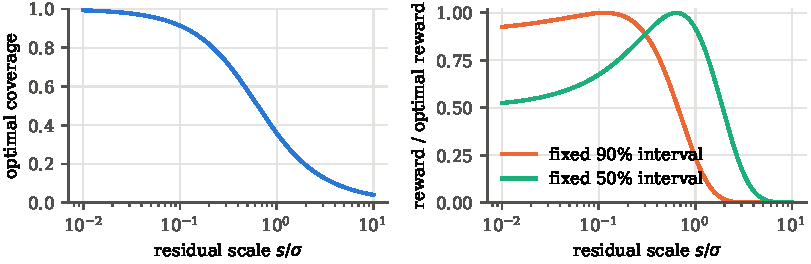
\includegraphics[width=\linewidth]{figs/sps_optimum.pdf}
\caption{The \sps{} optimum for a Gaussian residual of scale $s$ (analytic). \emph{Left:} coverage of the reward-optimal interval falls with $s/\sigma$. \emph{Right:} reward of fixed-coverage intervals relative to the optimum; each is optimal at a single scale.}
\label{fig:sps}
\end{figure}

\section{Method}
\label{sec:method}

\paragraph{Forecaster.} Each ensemble member is a 2-D convolutional network with time folded into channels: 20 frames of $(u,v)$ plus two coordinate channels are lifted by a $1\times1$ convolution to width 64, passed through 8 residual blocks $x+\mathrm{GN}(\mathrm{GELU}(\mathrm{pw}(x)+\mathrm{conv}_{3\times3}(x)+\mathrm{conv}_{5\times5,\mathrm{dil}=2}(x)))$, and decoded to 20 output frames added to the last observed frame (a delta parameterisation). A second head outputs a per-element log-scale. Each member has 1.16M parameters. Recipe~A maps 20 frames to 20 in one step; recipe~B applies a 20$\to$10 operator twice, feeding its own first 10 predictions back, with gradients through both steps. The submitted ensemble is two members of each recipe (seeds 250 and 350), 4.6M parameters in total. Inputs are z-scored with fixed global constants computed from the real training set.

\paragraph{Loss.} In physical units, with $r=y-\mu$ and $\shat=\exp(\text{scale head})$:
$\mathrm{relL2}(\mu,y)+0.15\,\mathrm{relL2}(\mathrm{TKE})+0.249\,\mathrm{MVPE}+3.0\,\overline{1-e^{-(r/2\shat)^2}}+0.2\,\mathrm{NLL}(r,\shat)$.
The coverage term detaches $\shat$ and trains $\mu$ to keep residuals inside the predicted scale; the NLL detaches $r$ and trains only the scale head. Training is 60,000 AdamW steps (learning rate $2\times10^{-3}$, one-cycle schedule, batch 32, bf16). Each network keeps its checkpoint with the best fixed composite of rel\_l2 and tke on two held-out Reynolds numbers.

\paragraph{Augmentation.} The incompressible Navier--Stokes equations are invariant under $u'(x,t)=k\,u(x,kt)$ at $\mathrm{Re}'=k^2\mathrm{Re}$. We draw $k$ log-uniform in $[0.75,1.6]$, resample each 40-frame window at times $kt$ by linear interpolation and scale the velocities by $k$. We also mirror across the cross-stream axis, negating $v$. Each transform is applied to 4 of every 32 windows.

\paragraph{Width table.}
\label{sec:width}
The predictive scale combines the members' own scales with their disagreement, $\shat^2=\overline{\exp(\mathrm{scale})^2}+0.75\operatorname{Var}_m(\mu_m)$. We bucket elements into 64 quantile bins of $\shat$ and, in each bin, take the exact empirical maximiser of $F(h)=e^{-2h/\sigma}\,\hat P(|r|\le h)$ over the sorted absolute residuals; the half-width is $0.95$ times the table interpolated at $\shat$. The residuals come from four \emph{cross-validation twins} trained with Reynolds numbers 13950 and 22875 held out, so the table never sees in-sample residuals. The factor $0.95$ and the disagreement weight were chosen by fitting on one held-out Reynolds number and scoring on the other, in both directions.

\paragraph{Variance head.} A conditional-mean forecaster under-predicts temporal fluctuation (\cref{sec:phase}). A degree-2 ridge model on seven window-local features predicts the log temporal variance of the true anomaly per pixel; the predicted anomaly is rescaled by $1+t(g-1)$ with $t=0.7$ where the gain $g\ge1$ and $0.2$ where $g<1$, only on pixels above the window's 70th percentile of predicted variance. All five post-hoc settings (the anomaly gain $1.05$, the three head settings and the width factor) are interior optima, bracketed on both sides.

\paragraph{Inference.} The four members run as one grouped-convolution trunk in fp16, with each block's $1\times1$ convolution folded into its $3\times3$ convolution. A CUDA graph is captured per batch-size bucket so that no call is padded, and outputs go through one pinned host buffer in fp16.

\section{Experimental protocol}
\label{sec:protocol}

\paragraph{Local validation.} The private test set holds unseen flow conditions, so the validation unit is a whole Reynolds number: all trajectories at Re 13950 and 22875 (8 trajectories, 336 non-overlapping windows) are held out, and our scorer mirrors the official one. Local levels were consistently optimistic relative to the hidden set (rel\_l2 by 1.7 points, \sps{} by 8.8). We therefore used local runs only to \emph{order} candidates, except where a matched-difficulty slice was validated against a hidden-test measurement (\cref{sec:results}).

\paragraph{Noise floors and pairing.} Three identical runs differ by $0.014$ standard deviation in rel\_l2 score; four seeds of the full recipe differ by $0.031$ in the assembled objective, almost all of it in tke and \sps{}. Unpaired deltas below $0.065$ are therefore unreadable. Every training-side comparison was seed-paired and required the same sign in both seeds and in both held-out directions. Post-hoc settings on a fixed network have no training variance and were compared exactly.

\paragraph{Oracle bounds and controls.} Where possible a candidate family was closed by an \emph{oracle} that is given information no deployable method has (the realised error on earlier frames, the true spectrum, the optimal displacement, the per-window best member); if the oracle cannot pay, no method in the family can. Each instrument carried a no-op control that must reproduce a known value bit-exactly, and where feasible a planted positive control that must be recovered.

\paragraph{Hidden-test submissions.} The board allowed one submission a day and kept each team's best entry. We used several of our 22 submissions as single-variable experiments with pre-registered predictions.

\section{Results}
\label{sec:results}

\begin{table}[t]
\centering
\caption{Final Track~1 ranking after organizer retraining on the private set (published 17~October~2026). Standard deviations are as published.}
\label{tab:final}
\small
\begin{tabular}{rlcc}
\toprule
Place & Team & Total score & Std.\ dev.\\
\midrule
1 & np-user & 82.9555 & 0.0281\\
2 & Pistachio & 82.9006 & 0.0166\\
3 & PhysicsOracle & 82.6085 & 0.0045\\
4 & syouya\_tobita & 82.5608 & 0.0223\\
5 & Aminos & 82.4877 & 0.0173\\
6= & skabob & 82.4434 & 0.0747\\
6= & AxisTilted2 & 82.4398 & 0.0319\\
8 & iapetos1918 & 82.4141 & 0.0226\\
\textbf{9} & \textbf{JLShen (ours)} & \textbf{82.3055} & \textbf{0.0061}\\
10 & Math4AI & 81.8406 & 0.1064\\
\bottomrule
\end{tabular}
\end{table}

\paragraph{Final standing.} On the development board our best entry scored $81.885$ (rel\_l2 94.849, tke 79.412, mvpe 93.941, time 91.537, \sps{} 44.309), 10th of 182. Its rel\_l2 was 2nd and its \sps{} 5th of the 182 entries. After the organizers' retraining on the private set it placed 9th with $82.3055$ and the second-smallest published standard deviation (\cref{tab:final}). Two independent from-scratch retrains of our recipe had scored $81.861$ and $81.846$ on the development board, so the result reflects the recipe, not a lucky draw.

\paragraph{Hidden-test trajectory.} \Cref{fig:ladder} shows all 22 hidden-test submissions. The largest step is submission 929156: the network weights and configuration of the previous best entry with only the width scale changed from $1.00$ to $0.65$. The four accuracy columns returned identical to the last digit, \sps{} rose from $40.556$ to $43.669$, and the final score from $80.856$ to $81.635$ (rank 33 to 7). Our matched-difficulty local slice had predicted an interval reward of $0.6147$ and a gain of $+0.782$; the board implied $0.6143$ and $+0.779$. The table that was replaced had been fitted on residuals passed through a heavy-tail correction model that we later found to be circular; measured against a refit on raw held-out residuals it was $1.24$--$1.97\times$ too wide, more so at small $\shat$, exactly as that correction model implies. The released pipeline refits the table on raw cross-validation residuals instead of rescaling the old one, which gave a further small gain.

\begin{figure}[t]
\centering
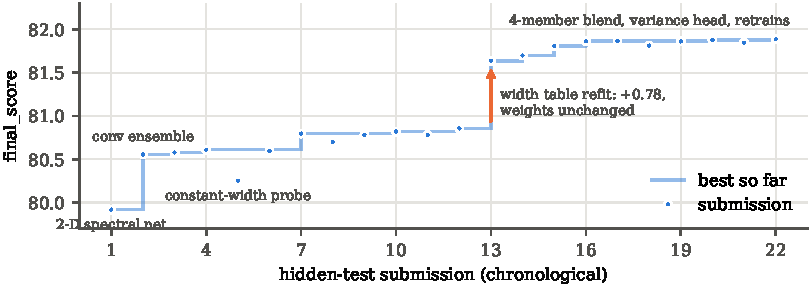
\includegraphics[width=\linewidth]{figs/ladder.pdf}
\caption{Final score of each hidden-test submission on the development board, in order. Submission 13 changes only the interval width; predictions are bit-identical to its predecessor's.}
\label{fig:ladder}
\end{figure}

\subsection{Where the ranking was decided}
\label{sec:where}

\Cref{tab:spread} attributes differences on the development board with the fitted weights. Against the median of 182 entries, our entry is ahead by $2.66$ points, and $1.82$ of them sit in \sps{}; within the top ten, \sps{} and time have the largest weighted spread. The \sps{} score mixes interval quality with accuracy through the factor $(1-p)$ in \cref{eq:sps}, but that factor varies little: inverting it, about $6.2$ of the median entry's $7.4$-point \sps{} deficit is interval quality. Accuracy is nearly saturated at the top: the ten best entries span $0.18$ in rel\_l2 score.

\begin{table}[t]
\centering
\caption{Development-board columns, attributed with the fitted aggregation weights. \emph{Top-10 range}: spread among the ten best entries. \emph{Top-10 vs median}: mean of the top ten minus the median of all 182 entries. Weighted columns are in final-score points.}
\label{tab:spread}
\small
\begin{tabular}{lcccccc}
\toprule
Column & Weight & Top-10 range & Weighted & Top-10 vs median & Weighted & Ours / rank\\
\midrule
rel\_l2 & 0.466 & 0.18 & 0.09 & 0.46 & 0.22 & 94.85 / 2\\
\sps{} & 0.246 & 1.02 & \textbf{0.25} & 7.41 & \textbf{1.82} & 44.31 / 5\\
tke & 0.102 & 1.14 & 0.12 & 2.56 & 0.26 & 79.41 / 20\\
mvpe & 0.105 & 0.36 & 0.04 & 0.90 & 0.10 & 93.94 / 32\\
time & 0.096 & 1.97 & 0.19 & 2.21 & 0.21 & 91.54 / 49\\
\bottomrule
\end{tabular}
\end{table}

\section{Findings}
\label{sec:findings}

\subsection{The width rule is at its information ceiling}

Once the width table is fitted on honest residuals, the class of rules $h=f(\shat)$ is exhausted: its in-sample oracle beats our cross-fitted table by $0.0007$ in reward on both held-out Reynolds numbers. Width adaptivity itself is worth a lot: on held-out residuals a single constant band reaches reward $0.614$ against $0.676$ for 64 buckets. But every attempt to sharpen $\shat$ stopped at the ceiling of \cref{sec:sps}: training the scale head on an \sps{} surrogate or on the median of $\log|r|$ instead of Gaussian NLL, a dedicated separate network for $|r|$, and extra per-element features. The strongest of these is an oracle that gives the width rule the model's \emph{realised} error on frames 1--10 when predicting frames 11--20; it adds $0.0004$ reward ($+0.008$ final). Asymmetric intervals searched on an $80\times80$ grid change the reward by $-0.0004$, and centring the interval on a different estimator than the scored prediction does not help.

\subsection{Simulation data did not help}
\label{sec:sim}

We tested three routes (\cref{fig:data}, left). \emph{Pretrain then finetune} gave $+0.0003$ interval reward and $+0.015$ rel\_l2, both inside the control's noise ($\approx+0.006$ final). \emph{Joint training} with the simulated windows re-expressed in real units, a fraction of each batch, lost monotonically in that fraction on every column and in both seeds: $-0.11$, $-0.46$ and $-0.99$ in the assembled objective at fractions $0.25$, $0.5$ and $0.75$. The tke column fell rather than rose, although the simulations carry about $3.6\times$ the fluctuation energy. \emph{Simulating the measurement}, by stamping a real window's own laser-obstruction mask onto each simulated window and adding white vector noise, cut the loss about fivefold, so the measurement process is the dominant part of the gap. Even so, the best fraction only reached zero ($-0.034$ and $+0.008$ in the two seeds at $0.25$). The noise, not the mask, carried the repair.

This disagrees with RealPDEBench's finding that simulation pretraining improves real-data accuracy~\citep{hu2026realpdebench}. The settings differ: our model is small and strongly augmented, the grid is subsampled, the horizon is 20 frames and the objective is the challenge composite. Our reading is that simulation pretraining helps when the real-data baseline is weak, and that a well-regularised real-only model with exact physical augmentation leaves nothing for it to add here. We did not try learned domain adaptation.

\begin{figure}[t]
\centering
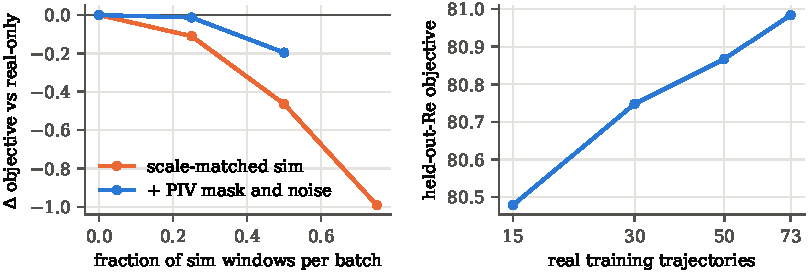
\includegraphics[width=\linewidth]{figs/data_regime.pdf}
\caption{\emph{Left:} change in the assembled held-out objective when a fraction of every batch is simulated data, scale-matched to real units, with and without simulating the PIV obstruction mask and noise (mean of two seeds). \emph{Right:} held-out objective against the number of real training trajectories, at fixed validation set.}
\label{fig:data}
\end{figure}

\subsection{The real-data regime}
\label{sec:regime}

\paragraph{Data-limited in trajectories, not capacity-limited.} A learning curve over whole trajectories (\cref{fig:data}, right) still climbs at 73 trajectories, roughly $0.3$ per $e$-fold, without flattening. Capacity is flat or harmful: a 2-D spectral net scored the same held-out rel\_l2 at 13M, 43M and 155M parameters, and a conv net with $4\times$ the parameters lost at full data, also when given twice the training steps. The 68k-window count overstates the effective sample size, which is closer to the number of independent trajectories. Supervising the three unscored subsampling phases of the full-resolution grid, $4\times$ more targets, lost monotonically with weight, because neighbouring phases of a smooth field are nearly redundant.

\paragraph{Physical augmentation pays.} Integer-stride Reynolds similarity ($k=2$) and the mirror compound only at a matched total dose: with each on $1/8$ of the batch they gained $+0.067$ in the assembled objective over no augmentation, $+0.016$ more than Reynolds similarity alone at the same total dose in both seeds, while doubling the dose lost. Replacing integer $k$ by continuous log-uniform $k\in[0.75,1.6]$ raised the gain over no augmentation to $+0.10$. Nearly all of it comes from $k<1$ (lower Reynolds numbers), which an integer stride cannot reach, and interpolating at exact similarity times beat snapping to the nearest frame. Plain noise augmentation and $k=3$ both lose.

\paragraph{Ensembling saturates at four near-clones.} Members are cheap in latency ($0.17$\,ms per sample each), but gains saturate at four, and seed clones beat recipe-diverse members of equal count because diversity cost more in member quality than it bought in decorrelation.

\subsection{The error is phase, not amplitude}
\label{sec:phase}

The model \emph{underfits}: its fluctuation energy is 70\% of the target's on training Reynolds numbers and the same on held-out ones, and its train and held-out rel\_l2 scores differ by only $0.06$. The 20-frame map is learnable: in a model-free test over 1920 pairs of similar held-out windows, output distance grows linearly with input distance (slope $1.22$, intercept zero within noise), so there is no irreducible noise floor at this horizon and resolution. Several families that target amplitude or registration are bounded by oracles. A semi-Lagrangian warp has an optimal shift of zero on 100\% of windows. Injecting the \emph{true} spatio-temporal spectrum with random phase, the ceiling of a generative or PDE-Refiner-style refiner~\citep{lippe2023pderefiner}, lowers the objective monotonically and leaves tke unchanged. Global spatial blurring or sharpening of the prediction loses in both directions. Per-window dynamic mode decomposition loses its phase within 3--7 frames, and analogue retrieval from the training corpus, although the most decorrelated predictor we measured, is bounded at $+0.16$ final score by a perfect per-element gate. What did help was recipe~B's autoregressive rollout of a 10-frame operator: $+0.05$ in the objective, with tke and rel\_l2 both up in both seeds; rollouts with shorter steps helped less or not at all. The post-hoc variance head recovers part of the amplitude deficit; it works because its gate removes estimator error, not signal.

\subsection{Latency was host bytes, not FLOPs}

The time column was charged on a shared evaluation host, and about 85\% of our charged time did not depend on FLOPs. One-copy output marshalling cut host work by 45\% with bit-identical output; padding a call of 5 windows to a 16-window graph tripled the forward work, fixed by per-bucket graphs; and fusing the four members into one fp16 grouped trunk made the forward pass $1.7\times$ faster. Together these moved the time score from $89.9$ to $92.0$ at best, about $+0.2$ final. Halving the output bytes again with fp16 was worth under 1\% once the pinned path was in place.

\section{Robustness and reproducibility}

The released pipeline trains all eight networks from the public data and refits the calibration; it has no network access and uses no pretrained weights. A full retrain inside the evaluation image (PyTorch 2.2.2), in place of our cluster environment (2.5.1), matched the cross-validation quality to $0.002$. On Reynolds numbers held out at the edge of the training range (25425, 26700) and on a whole held-out angle of attack, the post-hoc stack stayed positive at 20--40\% of its interior gain, and the width factor $0.95$ stayed within $0.006$ of the best setting. The released code is functionally identical to the submitted entry; \cref{app:release} describes how we verified this.

\section{Limitations}

All findings come from one dataset, one grid and one 20-frame horizon, and from the challenge composite rather than a physics-oriented metric. Local levels did not transfer to the hidden set, so most local findings are orderings; the hidden-test measurements are few and some cannot be separated from evaluation-host noise in the time column. The simulation results cover three routes and not learned domain adaptation. The aggregation weights are fitted, not published. The experiment programme was run with an autonomous LLM-agent harness under the author's supervision (see Acknowledgements); every number in this report was produced by logged code and checked against the logged record, but the record is the agent's.

\section{Conclusion}

In a challenge framed as Sim2Real, our top-10 entry used no simulation data, and controlled tests say that simulation data would not have helped it. What separated entries was largely the calibration of the uncertainty intervals, under a score whose optimum is not a fixed-coverage interval and which rewards abandoning hard elements. For benchmark designers, the lesson is that such a score makes calibration plumbing worth more than modelling; a proper interval score would reward the predictive distribution itself. For participants, the lessons are to fit post-hoc calibration on honest held-out residuals, to treat the number of independent trajectories rather than frames as the sample size, and to look for exact physical symmetries before larger models or more data of a different kind.

\paragraph{Code.} \url{https://github.com/jlshen025/competition_solutions/tree/main/realpde_t1}

\paragraph{Acknowledgements.} We thank the RealPDE organizers for the data, the evaluation platform and the retraining effort. Compute was provided by the Digital Research Alliance of Canada (nibi). The experiments were planned, run and logged by AutoAgent, an autonomous LLM-agent harness developed by the author, which also consulted other LLMs for ideas; the author set the objectives and rules, reviewed the record and wrote this report with AI assistance.

\bibliographystyle{plainnat}
\bibliography{refs}

\appendix

\section{Selected ruled-out levers}
\label{app:levers}

\begin{table}[h]
\centering
\caption{A selection of the 101 ruled-out levers. Effects are on the assembled held-out objective or the interval reward $F$, seed-paired; ``oracle'' marks a bound from information no deployable method has.}
\small
\begin{tabular}{p{0.38\linewidth}p{0.55\linewidth}}
\toprule
Lever & Evidence\\
\midrule
Wider/deeper spectral or conv nets & Flat over 13M--155M; $4\times$ width loses at $2\times$ steps\\
Sim pretraining; joint sim+real & $+0.006$ final (noise); monotone loss to $-0.99$\\
Supervise unscored grid phases & Monotone loss with weight\\
EMA/SWA weight averaging & Neutral on rel\_l2\\
Distil the ensemble into one net & Below the ensemble at equal teacher set\\
Recipe-diverse members; more than 4 members & Seed clones win; 6 members negative after latency\\
Semi-Lagrangian warp decoder & Oracle shift $(0,0)$ on 100\% of windows\\
Spectrum-matching refiner (PDE-Refiner, diffusion) & Oracle: monotone loss, tke unchanged\\
DMD phase extrapolation; analogue retrieval & Oracle gate $\le+0.16$ final; every blend loses\\
Spatial sharpening or blurring & Interior optimum at zero, both sides\\
Multiscale (U-shaped) trunk & Worst of twelve architecture arms\\
\sps{} surrogate or median loss for the scale head & Same $F$ as NLL; lower rank correlation\\
Extra per-element width features & Oracle with realised error: $+0.0004$ $F$\\
Asymmetric or re-centred intervals & $-0.0004$ $F$; mean is the best centre\\
Per-window self-normalised scale & Loses in both directions\\
Spectral power-matching loss & Monotone loss over a $100\times$ dose range\\
Incompressibility projection & 2-D divergence is 64\% of vorticity (3-D flow)\\
\bottomrule
\end{tabular}
\end{table}

\section{Release verification}
\label{app:release}

The submitted package carried exploratory options that the shipped configuration never reaches; the public release removes them (\texttt{train.py} shrinks from 1501 to 305 lines). On an H100 MIG slice we checked the cleaned against the submitted code on the submitted configuration. Preprocessing writes byte-identical arrays. Assembling the archive from the same four checkpoints and calibration fits gives a byte-identical \texttt{config.json} and checkpoints. Predictions and bounds are bitwise identical for batch sizes 1, 5, 7, 16, 23 and 70. The width-table and variance-head fits write byte-identical results. 1000 training steps of each recipe from the same seed give bitwise-identical weights and loss logs. The cleaned code calls no PyTorch API the submitted code did not. A 50-step run of the full \texttt{train} entry point completes and returns valid bounds. These checks used synthetic data in the release format; a full 60,000-step run on the real data was not repeated.

\end{document}
